\section{口令协议:针对直接攻击的安全性}\label{sec:18-3}

在\textbf{基本口令协议 (Basic Password protocol)}中,证明者的密钥是一个\textbf{口令} $pw$。在该协议中,证明者将 $pw$ 发送给验证者,验证者需要检查 $pw$ 是否是合法的口令。因此,该协议的密钥 $sk$ 就是 $pw$。显然,只有当对手无法窃听证明者和验证者之间的交互时,这个协议才可以被使用。为了完善对基本口令协议的定义,我们还需要指定验证者如何检查给定的口令是否合法。

首先想到的方法是直接将验证者的公钥也定义为 $vk:=pw$,这样验证者只需要检查它从证明者那里收到的口令与 $vk$ 是否相等即可。但是这种简陋的协议显然是有问题的,因为如果验证者被攻破,所有验证者存储的口令都会直接泄露。

为了避免这个问题,我们可以让验证者保存口令的哈希值,而不是口令本身。我们称这个修改后的口令协议为\textbf{版本 1}。我们下面用一种相当理想化的方式来描述这个协议,在该协议中,我们从某个有限的口令空间中随机均匀地选择口令,但实际情况可能并非如此。

\begin{snote}[口令协议版本 1.]
证明者的私钥 $sk$ 是一个从有限口令空间 $\mathcal P$ 中随机均匀选出的口令 $pw$,验证者的公钥 $vk=H(pw)$,其中的哈希函数为 $H:\mathcal{P}\to\mathcal{Y}$。这样,\textbf{口令身份认证协议} $\mathcal{I}_{\rm pwd}=(G,P,V)$ 的定义如下:
\begin{itemize}
    \item $G$:令 $pw\xleftarrow{\rm R}\mathcal{P}$ 并输出 $sk=pw$ 和 $vk=H(pw)$。
    \item 以 $sk=pw$ 为输入的算法 $P$ 及以 $vk=H(pw)$ 为输入的算法 $V$,它们按照以下方式交互:
    \begin{enumerate}
        \item $P$ 将 $pw$ 发送给 $V$;
        \item 如果收到的 $pw$ 满足 $H(pw)=vk$,$V$ 输出 $\mathsf{accept}$,否则输出 $\mathsf{reject}$。
    \end{enumerate}
\end{itemize}

在一个多用户系统中,验证者(服务器)通常会在数据库中维护一张口令映射表,就像图 \ref{fig:18-2} 一样。因此,对服务器的攻击不会泄露出任何的明文口令。

为了分析上述口令协议的安全性,我们下面首先正式定义针对直接攻击的安全性,然后解释为什么上面的协议能够满足这个安全定义。
\end{snote}

\begin{figure}
    \centering
    

\tikzset{every picture/.style={line width=0.75pt}} %set default line width to 0.75pt        

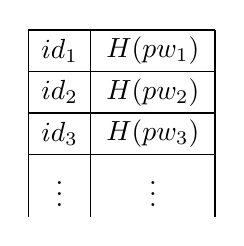
\begin{tikzpicture}[x=0.75pt,y=0.75pt,yscale=-1,xscale=1]
%uncomment if require: \path (0,94); %set diagram left start at 0, and has height of 94

%Straight Lines [id:da6400294958570547] 
\draw  [line width=0.5]  (0,0) -- (0,90) ;
%Straight Lines [id:da9802107235934225] 
\draw  [line width=0.5]  (0,0) -- (90,0) ;
%Straight Lines [id:da6980864355891092] 
\draw  [line width=0.5]  (30,0) -- (30,90) ;
%Straight Lines [id:da5983629013813236] 
\draw  [line width=0.5]  (90,0) -- (90,90) ;
%Straight Lines [id:da4382498247103943] 
\draw  [line width=0.5]  (0,20) -- (90,20) ;
%Straight Lines [id:da45190507971026106] 
\draw  [line width=0.5]  (0,40) -- (90,40) ;
%Straight Lines [id:da8316323031260375] 
\draw  [line width=0.5]  (0,60) -- (90,60) ;

% Text Node
\draw (15,10) node    {$id_{1}$};
% Text Node
\draw (15,30) node    {$id_{2}$};
% Text Node
\draw (15,50) node    {$id_{3}$};
% Text Node
\draw (15,75) node    {$\vdots $};
% Text Node
\draw (60,10) node    {$H( pw_{1})$};
% Text Node
\draw (60,75) node    {$\vdots $};
% Text Node
\draw (60,30) node    {$H( pw_{2})$};
% Text Node
\draw (60,50) node    {$H( pw_{3})$};


\end{tikzpicture}
    \caption{储存在服务器中的口令文件(版本1)}
    \label{fig:18-2}
\end{figure}

\begin{game}[针对直接攻击安全的身份识别]\label{game:18-1}
对于一个给定的身份识别协议 $\mathcal{I}=(G,P,V)$ 和一个给定对手 $\mathcal{A}$,攻击游戏按照以下方式运行:
\begin{itemize}
    \item 密钥生成阶段。挑战者运行 $(vk,sk)\xleftarrow{\rm R} G()$ 并将 $vk$ 发送给 $\mathcal{A}$。
    \item 仿冒尝试阶段。挑战者与 $\mathcal{A}$ 交互,其中挑战者掌握 $vk$,并按照验证者的算法 $V$ 运行,而对手 $\mathcal{A}$ 扮演证明者的角色,但不一定会诚实执行证明者的算法 $P$(事实上 $\mathcal{A}$ 根本没有获取到私钥 $sk$)。
\end{itemize}
如果 $V$ 在交互结束时输出 $\mathsf{accept}$,我们就称对手 $\mathcal{A}$ 赢得了本游戏。我们定义 $\rm{ID1\mathsf{adv}}[\mathcal{A},\mathcal{I}]$ 为对手 $\mathcal{A}$ 相对 $\mathcal{I}$ 的优势,其值为 $\mathcal{A}$ 赢得本游戏的概率。{\hfill $\square$}
\end{game}

\begin{definition}\label{def:18-2}
如果对于任意有效对手 $\mathcal{A}$,$\rm{ID1\mathsf{adv}}[\mathcal{A},\mathcal{I}]$ 的值都可以忽略不计,我们就称身份识别协议 $\mathcal{I}$ \textbf{对于直接攻击是安全的}。
\end{definition}

请注意,在游戏 \ref{game:18-1} 中,对手 $\mathcal{A}$ 能够获得的是验证密钥 $vk$。因此,一个将明文口令直接存储的简陋口令协议并不满足定义 \ref{def:18-2}。下面的简单定理表明,版本1的协议是安全的。

\begin{theorem}\label{theo:18-1}
如果哈希函数 $H:\mathcal{P}\to\mathcal{Y}$ 是单向的,那么口令协议 $\mathcal{I}_{pwd}$ 针对直接攻击是安全的。
\end{theorem}

\begin{proof}[证明简述]
为了攻击协议 $\mathcal{I}_{pwd}$,对手 $\mathcal{A}$ 必须能够提供一个口令 $pw'$ 使得 $H(pw')=H(pw)$。需要注意的是 $pw'$ 可能与 $pw$ 不同。而能够提供满足上述要求的 $pw'$ 的对手显然已经破坏了 $H$ 的单向性。
\end{proof}

我们可以注意到,针对直接攻击(见攻击游戏 \ref{game:18-1})的安全性事实上是一个非常弱的安全概念。比如说,尽管口令协议 $\mathcal{I}_{pwd}$ 对于直接攻击是安全的,但是对手哪怕能够窃听到协议的一个实例,它显然就丧失了安全性。

\subsection{利用字典攻击破解口令}

口令协议 $\mathcal{I}_{pwd}$ 在实践中被广泛使用,因为它使用起来非常方便。任何人只要记住一个口令 $pw$,就可以参与到协议中来,扮演证明者的角色,并且不需要任何额外的计算设备。问题是,人类生成和记忆随机口令的能力是在太过糟糕。在实践中,被使用的口令通常太短了。更糟糕的是,口令通常根本就不是随机生成的,而是根据一些可预测的信息推导来的。

\begin{figure}
    \centering
    \tikzset{every picture/.style={line width=0.75pt}}   

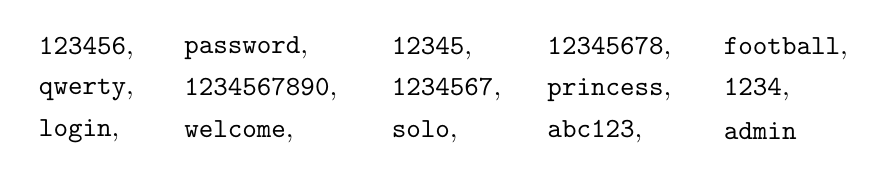
\begin{tikzpicture}[x=0.75pt,y=0.75pt,yscale=-1,xscale=1]

\draw (0,10) node [anchor=west] [align=left] {\texttt{123456},};
\draw (70,10) node [anchor=west] [align=left] {\texttt{password},};
\draw (170,10) node [anchor=west] [align=left] {\texttt{12345},};
\draw (245,10) node [anchor=west] [align=left] {\texttt{12345678},};
\draw (330,10) node [anchor=west] [align=left] {\texttt{football},};

\draw (0,30) node [anchor=west] [align=left] {\texttt{qwerty},};
\draw (70,30) node [anchor=west] [align=left] {\texttt{1234567890},};
\draw (170,30) node [anchor=west] [align=left] {\texttt{1234567},};
\draw (245,30) node [anchor=west] [align=left] {\texttt{princess},};
\draw (330,30) node [anchor=west] [align=left] {\texttt{1234},};

\draw (0,50) node [anchor=west] [align=left] {\texttt{login},};
\draw (70,50) node [anchor=west] [align=left] {\texttt{welcome},};
\draw (170,50) node [anchor=west] [align=left] {\texttt{solo},};
\draw (245,50) node [anchor=west] [align=left] {\texttt{abc123},};
\draw (330,50) node [anchor=west] [align=left] {\texttt{admin}};

\end{tikzpicture}
    \caption{依次列出的2016年中最常见的15个口令}
    \label{fig:18-3}
\end{figure}

图 \ref{fig:18-3} 总结了2016年进行的一项研究的结果,该研究检查了500万个泄露的口令,这些口令大多由北美和西欧的用户持有。数据显示,这些口令与大集合上的均匀分布相去甚远,尤其是有相当比例的口令属于相对较小的常用口令字典。大约4\%的人使用``123456"这个口令,而大约10\%的人使用前25个最常用口令列表中的某一个。图 \ref{fig:18-3} 中的口令列表在一段时间内非常稳定。每年的变化都非常小。

从现在开始,我们使用\textbf{强口令}来表示从一个很大口令空间 $\mathcal{P}$ 中随机均匀选出的口令。只有口令是强口令时,定理 \ref{theo:18-1} 的安全性声明才有效。相对地,\textbf{弱口令}就是指那些从一些常用口令的小字典中按照某个任意分布选取的口令。我们将弱口令的口令空间表示为 $\mathcal{D}$,则必然有 $\mathcal{D}\subseteq\mathcal{P}$。

\subsubsection{在线字典攻击}

假设现在有一个对手怀疑某个用户的口令很弱,属于某个常用口令的小字典 $\mathcal{D}$。那么对手就可以发动一个\textbf{在线字典攻击}:它只需要逐一尝试 $\mathcal{D}$ 中的所有口令,直到找到匹配的口令。为了进一步提升效率,对手可以按照流行程度对 $\mathcal{D}$ 中的元素进行排序,首先尝试更流行的口令。

一个常见的防御在线字典攻击的方法是,在特定用户 ID 或来自特定 IP 地址的登录尝试每两次失败后,就将服务器的响应时间增加一倍。因此在十次登录失败后,下一次尝试的时间就会是正常响应时间的 $32$ 倍。即使一个用户并不能熟记自己的口令,它也不过需要等待一点时间,所以对它来说这种设计的影响并不大。但是对于恶意攻击者来说,通过暴力破解的方式去猜测口令会变得非常困难。

对手为了应对这种反制对策,可以在许多不同的用户名中尝试同一个普通的口令,比如 $\mathtt{123456}$。此外,对手可以利用位于不同 IP 地址的肉机来反制对于单个 IP 地址的登录尝试次数限制。用这种方式对随机账户进行攻击对于一般的对手来说往往已经足够了,他们通常会在地下论坛中交易攻击得到的数据。

非密码学的防御手段对于阻吓这些在线攻击已经很有效了。但是仍然有更具破坏性的攻击,这种攻击也更难阻止。我们将在接下来讨论这种攻击。

\subsubsection{离线词典攻击}\label{subsubsec:18-3-1-2}

攻击者如果破坏了登录服务器,就可以窃取存储在服务器上的口令数据库。这给了攻击者一个大的哈希口里ing列表,每个在该系统注册的用户都有一个口令。

侵入登录服务器的对手可以窃取服务器上存储的口令数据库,攻击者可以借此得到大量哈希后的口令。除了直接破坏服务器外,还有许多其他方法可以获得口令文件。例如一项研究表明,在eBay上购买的二手硬盘可以包含很多有趣的、未被删除的数据,其中就包括口令文件。

现在假设一个对手设法获得了某个用户的验证密钥 $vk=H(pw)$。如果口令 $pw$ 是弱的,并且属于某个常见口令的小字典 $\mathcal{D}$,那么对手就能够发动\textbf{离线字典攻击},它可以这么做:
\begin{equation}\label{eq:18-1}
	\begin{aligned}
		& \text{对每个~}w\in\mathcal{D}:\\
		& \text{~~~~~~~~如果~}H(w)=vk:\\
		& \text{~~~~~~~~~~~~~~~~输出~} w \text{ 并停机}
	\end{aligned}
\end{equation}
如果 $pw$ 在 $\mathcal{D}$ 中,那么依照上述过程,对手迟早能够获取 $pw$,抑或是另一个 $pw'$ 使得 $H(pw')=H(pw)$。

这种离线字典攻击的时间复杂度是 $O(|\mathcal{D}|)$,其中时间单位为对一个输入计算一次$H$的耗时。这种计算完全可以\emph{脱机}运行,不需要与证明者或服务器有任何交互。

\begin{snote}[口令统计.]
2016年,一个名为 CrackStation 的口令破解服务发布了一个大小约为 15 亿的的常用口令词典。经验证据表明,人类生成的口令中有接近 50\% 都在这个列表中。这意味着,每经过约 15 亿次的离线哈希,每两个口令中就有一个能被破解。如果哈希函数 $H$ 是 SHA256,那么现代 GPU 只需要不到一分钟的时间就能够完成破解。由此我们能够得出一个结论:简单地使用 SHA256 对口令进行哈希处理对保护口令数据来说远远不够。

从另一个角度来说,我们可以发现,只包含可打印字符的 8 位字符口令的总数大约是 $95^8 \approx 2^{52}$ 个,这是因为美式键盘上有 95 个可输入字符。使用现代 GPU 阵列对这组口令中的所有单词运行 SHA256 也不过仅仅几天就可以完成。这说明,\emph{所有}8位以下长度口令在服务器被攻破的情况下都是不安全的。
\end{snote}

\begin{snote}[量子离线口令攻击.]
更糟糕的是,一旦有了大规模的量子计算机,上面的穷举搜索攻击将会更加容易。我们在4.3.4节中介绍过,量子计算机可以在 $\sqrt{n}$ 级别的时间内搜索大小为 $n$ 的空间。因此对于 8 位长度的口令空间来说,量子搜索相当于只需要进行 $\sqrt{2^{52}}=2^{26}$ 次哈希计算。这在现代经典计算机上也仅仅需要几秒钟而已。换言之,由于 8 位长度口令在经典计算机上是不能抵抗穷举搜索的,所以一旦我们拥有一台在速度和大小上与当前经典计算机相当的量子计算机,16 位长度的口令也将失去安全保障。我们将在18.4.3节中讨论一些针对该问题防御措施。
\end{snote}

\subsubsection{含预处理的离线字典攻击}

如果对手能够在发动攻击之前对字典 $\mathcal{D}$ 进行预处理,那么上面讨论的离线字典攻击将会更容易发动。一旦获取了哈希后的口令 $vk$,对手就能够立即从字典中查到原始口令 $pw$。具体来说,我们可以将字典攻击分为两个阶段:一个\textbf{预处理阶段},在获取任何哈希口令之前发动;一个\textbf{攻击阶段},针对特定口令$vk$发起攻击。我们的目标是尽量减少攻击阶段破解特定 $vk$ 所需的时间。

一个简单的带有预处理阶段的字典攻击原理如下:
\begin{equation}\label{eq:18-2}
	\begin{aligned}
		& \text{预处理阶段}:\\
		& \text{~~~~~~~~对于每个~}pw\in\mathcal{D}\text{,将~}(pw,H(pw))\text{~加入列表~}L\\
		& \text{针对输入~}vk\text{~的攻击阶段}:\\
		& \text{~~~~~~~~如果在表~}L\text{~中存在一项~}(pw,vk)\text{,则输出~}pw\\
		& \text{~~~~~~~~否则输出~}\mathsf{fail}
	\end{aligned}
\end{equation}
假设我们把对一个口令计算一次$H$的耗时作为时间单位,那么预处理阶段所需要的时间为 $O(|\mathcal{D}|)$级。如果表 $L$ 存储在一个支持常数时间查找的哈希表中,那么攻击阶段将会非常快,耗时仅仅为常数级。

\begin{snote}[批量离线字典攻击.]
一旦完成预处理,攻击者就能利用它快速破解许多哈希口令。具体来说,假设攻击者从一个被攻破的登录服务器中获得了一个大型的哈希口令数据库 $F$,那么现在使用字典 $\mathcal{D}$ 破解 $F$ 中的哈希后口令仅需要:
\begin{equation}
	\begin{aligned}
		& \text{预处理阶段:}O(|\mathcal{D}|)\\
		& \text{攻击阶段:}O(|F|)
	\end{aligned}
\end{equation}
其中 $|F|$ 指 $F$ 中哈希口令的数量。上述批量离线字典攻击的总工作量是 $O(|\mathcal{D}|+|F|)$,这比针对 $F$ 中每一个元素分别单独发起式 \ref{eq:18-1} 的离线字典攻击要快得多,因为后者的总工作量是 $O(|\mathcal{D}|\times |F|)$。

回忆一下,\ref{subsubsec:18-3-1-2} 节中的统计数据表明,对手可以使用 CrackStation 字典找到 $F$ 中近\emph{半数}的口令。因此一旦完成预处理,只需要 $O(|F|)$ 时间就能完成攻击。事实上这种攻击能够使用极少的工作量暴露数百万个被破解的口令。
\end{snote}

\begin{snote}[时空权衡.]
式 \ref{eq:18-2} 所展示的基于预处理的字典攻击要求攻击者建立并存储一个包含大量哈希口令的列表 $L$。然而当字典 $\mathcal{D}$ 是所有 $2^{52}$ 个 8 字符口令的集合时,这个表 $L$ 可能会相当大,存储成本过高。在第18.7节中,我们会介绍一种名为\textbf{彩虹表}的方法,它在预处理阶段构建一个小得多的表$L$,并用它快速破解口令。比如说,在 $n:=|\mathcal{D}|$ 的情况下,该方法能够实现:
\begin{equation*}
	\begin{aligned}
		& \text{表大小:}O(n^{2/3})\\
		& \text{预处理时间:}O(n)\\
		& \text{攻击时间:}O(n^{2/3})
	\end{aligned}
\end{equation*}
表的大小从 $O(n)$ 缩减到 $O(n^{2/3})$ 级别。然而,攻击一个哈希口令的时间从 $O(1)$ 级增长到 $O(n^{2/3})$ 级。换言之,我们用更长的攻击时间换取了表 $L$ 大小的缩减。正因此,这种方法被称为\textbf{时空权衡}。我们通常不讨论预处理阶段的耗时,因为预处理是一个一次性过程,它在攻击开始之前就完成了。

这种时空权衡进一步说明了为什么简单地存储哈希口令是错误的做法。我们将在之后讨论针对性的防御措施。
\end{snote}